% IE 643 novelty-assessment report (max 2 pages), in the style of the intensive-assessment report (report_IE643.pdf).
% Build from this folder: pdflatex report.tex (twice). Numbers come from STUDIES.md (study numbers in the text) and results/.
\documentclass[10pt,a4paper]{article}
\usepackage[a4paper,margin=1.5cm,top=1.2cm,bottom=1.2cm]{geometry}
\usepackage[T1]{fontenc}
\usepackage[utf8]{inputenc}
\usepackage{lmodern}
\usepackage{graphicx,booktabs,enumitem,caption,titlesec,xurl,tabularx,array}
\captionsetup{font=small,labelfont=bf,skip=2pt}
\titleformat{\section}{\large\bfseries}{\thesection}{0.6em}{}
\titlespacing*{\section}{0pt}{6pt}{2pt}
\titleformat{\subsection}{\normalsize\bfseries}{\thesubsection}{0.5em}{}
\titlespacing*{\subsection}{0pt}{3pt}{1pt}
\setlist{nosep,leftmargin=1.3em}
\setlength{\parindent}{1.1em}\setlength{\parskip}{0pt}
\pagestyle{empty}
\newcolumntype{L}{>{\raggedright\arraybackslash}X}

\begin{document}
\begin{center}
{\Large\bfseries Cross-Template Key-Value Field Extraction from Scanned Forms}\\[2pt]
{\large\bfseries Novelty Assessment Report}\\[2pt]
IE 643 Course Project \quad Team: Unemployed and Unsupervised\\[1pt]
Param Mehta (23b2439) \quad Arjoe Basak (23b1295) \quad Indian Institute of Technology Bombay \quad 22 November 2026
\end{center}
\vspace{-4pt}
\begin{center}\begin{minipage}{0.93\linewidth}\small
\textbf{Abstract.} We extract named fields and key-value pairs from scanned forms whose template the model has never seen. After the intensive phase, our best trained model was BROS with sliding windows (92.4 F1 on seen templates, 71.3 on unseen ones). The novelty phase asks four questions. Can a zero-shot vision-language reader, which reads field names, beat the trained tagger on new wording? How well does key-value linking really work when measured end to end? Do tables fit the same pipeline? Do page pixels help? A grounded zero-shot reader scores 76.5 against 70.5 for BROS, but training wins once about 10 templates are seen and on tables. End-to-end linking rises from 47.4 to 53.4 with BROS, and falls with a multilingual encoder. Code: \url{https://github.com/ABasakEE/KeyValue-Extraction}.
\end{minipage}\end{center}

\section{Introduction}
A deployed form reader keeps meeting forms it was not trained on: a new vendor, a revised filing. Random splits hide this: a model can remember where each field usually sits. Our protocol holds out whole templates: VRDU [3] registration forms, 200 training documents, three folds, scored by exact-span entity F1; MTL keeps every template in training and UTL holds one out. An error analysis of the intensive phase put most of the unseen-template loss in two fields. \emph{foreign\_principle\_name} scored 0--13 F1 for every trained model, because each template words it differently, and on Short-Form 95\% of the wrong \emph{registrant\_name} predictions were the filer block. A tagger trained on 200 documents cannot learn which text a field name refers to, so we tried models that read field names. Each study was registered in \texttt{STUDIES.md} with its pass rule first.

\section{Approaches and experiments}
\begin{table}[h]\centering\footnotesize
\caption{Summary of the novelty-phase studies (S = study number in \texttt{STUDIES.md}).}
\begin{tabularx}{\linewidth}{@{}p{1.15cm}p{4.6cm}Lp{2.4cm}@{}}
\toprule
Study & Approach & Main result & Verdict \\
\midrule
S6--12 & Zero-shot VLM (3B) with a per-field router & router $+3.8$ F1 [$+2.6$, $+5.0$] over BROS on 300 fresh forms & passed \\
S25, 31 & Grounded prompt, Qwen3-VL-8B; prompt v2 & 76.5 / 75.2 vs BROS 70.5 / 69.8; with router 79.2 & helps (prompt tuned) \\
S29 & LoRA fine-tuning of the 3B VLM & 46.2 vs 70.1 for BROS & worse \\
S33 & Reader vs BROS trained on $K$ FATURA templates & reader wins at $K{=}1,2$, ties at 5, BROS wins at 10, 40 & crossover \\
S17--23 & Re-measure XFUND linking & 65.5 $\to$ 49.9 $\to$ 47.7 end to end & correction \\
S24, 26, 37 & Multilingual text; crops; BROS backbone & 47.7 $\to$ 44.2; 47.4 $\to$ 49.7; 47.4 $\to$ \textbf{53.4} & worse; helps; better \\
S34--41 & Line items: BROS tagger + anchor rule & ad-buy 68.8--85.7 row F1; DocILE \textbf{59.6} (whole pool 60.4) & works \\
S35, 40, 43 & Learned row grouper; column rules; VLM typer & $-4.3$; $-2.7$ / $+0.0$; $-7.45$ row F1 & not adopted \\
S42 & LayoutLMv3, page image vs blank image & unseen 63.8 vs 60.4; seen 92.2 vs 92.4 & helps, marginal \\
\bottomrule
\end{tabularx}
\end{table}

\subsection{A zero-shot reader for unseen wording (S6--12, 25, 29, 31)}
We first ran Qwen2.5-VL-3B zero-shot on the page and mapped its keys to our fields. Under a strict matched metric BROS [1] stayed ahead, but the errors were complementary: the VLM was better on role fields, BROS on dates, signatures and span boundaries. We then built a schema-guided, grounded recipe [5]: the model sees each page's OCR lines with ids and a short description of each field, answers in JSON by copying the value and citing its line, and we ground the answer back to OCR words. With prompt v2, Qwen3-VL-8B [6] in 4-bit reached \textbf{76.5 / 75.2} on the confirm and dev sets against 70.5 / 69.8 for BROS; text alone gives 73.3 / 71.7, so the image adds about 3 points. The router reaches 79.2 but loses 4.6 on Amendment. The prompt was changed after we saw dev and confirm results, and the replication on 300 untouched forms (S32) did not run, so the gain carries that caveat. Fine-tuning the 3B model with LoRA made it worse (46.2).

\subsection{Where training wins (S18, 33, 34, 38, 43)}
On FATURA invoices the recipe scores 91.7; BROS trained on $K = 1, 2, 5, 10, 40$ templates scores 32.5, 69.2, 90.8, 95.9, 99.9. The reader wins at $K = 1, 2$ ($+59.4$, $+22.5$), ties at 5, and loses at 10 and 40 (Figure~1). On tables it loses at every size: 38.2 row F1 on VRDU ad-buy against 68.8--85.7 for BROS, and on DocILE its pilot failed the output-format gate. As a field typer on top of BROS's DocILE cells the VLM cost 7.45 row F1, with typing accuracy 46--52\% against 77\%. The two systems fail together (the VLM is right on 32\% of the spans BROS misses, 70\% of those BROS gets right), so a confidence gate added nothing.

\subsection{Key-value linking, measured end to end (S17--24, 26, 27, 37)}
The intensive-phase linker reported 65.5 link F1 on XFUND. That scored only the 61\% of links visible in 512 tokens and gave the linker gold entities. Counting cut-off links as misses gives 49.9, and fully end to end, with predicted entities, the score is 47.7 (47.4 when the same LiLT [2] recipe was retrained later). XFUND validation is about 94\% sibling-free, close to a template-disjoint test. LiLT's multilingual text stream lowered link F1 by 3.5 in all three seeds; link-preserving crops raised it to 49.7; replacing LiLT by BROS, which encodes relative layout, raised it to 53.4 (entity F1 75.8 $\to$ 80.2; answers above their question $+15.4$ recall). Most linking errors are geometric (downward and question-to-question links). BROS is English-only, so the gain appears despite the language mismatch.

\subsection{Tables in the same pipeline (S34--41, 44) and page pixels (S42)}
A table row is another linking problem: detect cells as word sets, then attach each cell to the nearest anchor cell at or above it. With gold cells this rule reaches 94.4 row F1 on DocILE [4], our ceiling. With the unchanged BROS tagger, unseen-layout row F1 is 44.7 / 52.9 / 59.6 at 50 / 200 / 1,000 training documents and 60.4 on the whole pool, level with the published RoBERTa baseline on unseen layouts (59.8; different test documents). Seen layouts score 65.9, a gap of 2--9 points against 21 on VRDU forms. On unseen layouts 64\% of gold cells are right, 21\% missed, 8\% typed wrongly, 5\% wrongly bounded. LayoutLMv3 with and without the page image scores 92.24 and 92.35 on seen templates, and 63.8 and 60.4 on unseen ones (folds 0 and 1: the image adds $+3.4$, on the signature fields, with one unstable seed), 14--17 points below Track-1 BROS, which also uses anchoring and jitter.

\section{Qualitative results}
\begin{figure}[h]\centering
\begin{minipage}[t]{0.40\linewidth}\centering
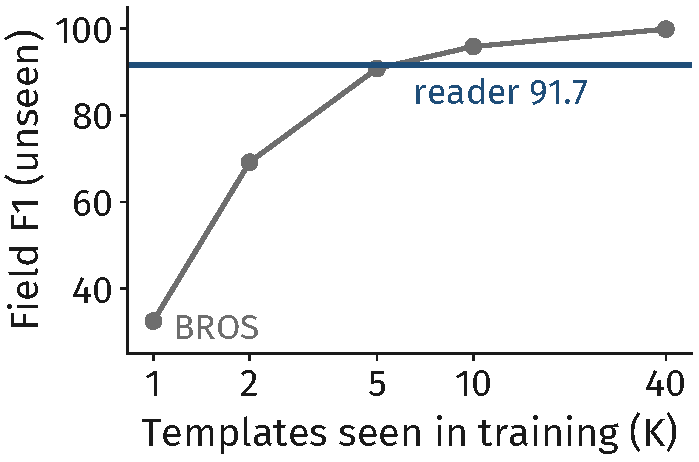
\includegraphics[width=\linewidth]{../poster/figures/f2_fatura_crossover.pdf}
\end{minipage}\hfill
\begin{minipage}[t]{0.40\linewidth}\centering
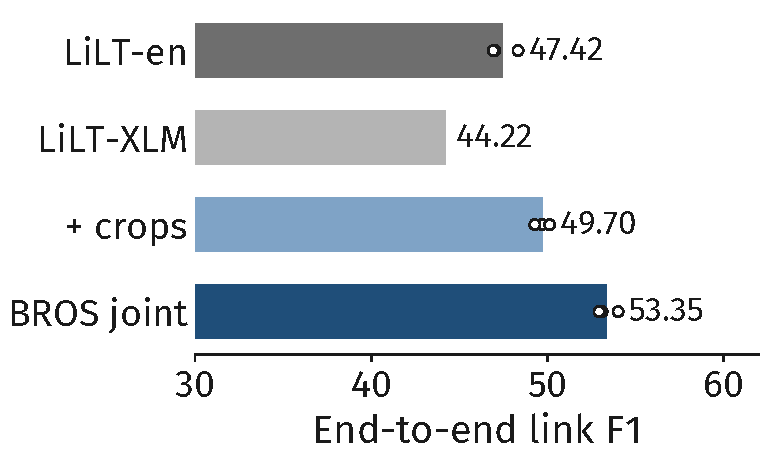
\includegraphics[width=\linewidth]{../poster/figures/f3_xfund_links.pdf}
\end{minipage}\\[4pt]
\begin{minipage}[t]{0.49\linewidth}\centering
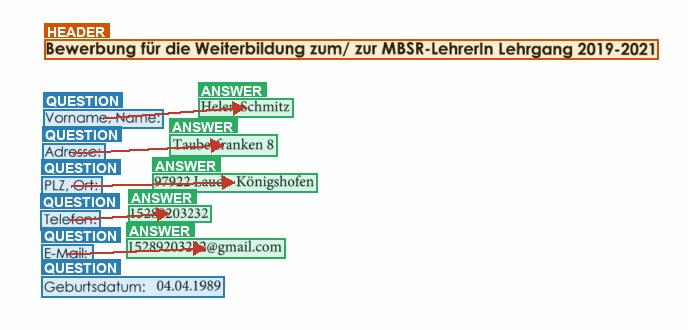
\includegraphics[width=\linewidth]{figures/linking_example_de.png}
\end{minipage}\hfill
\begin{minipage}[t]{0.49\linewidth}\centering
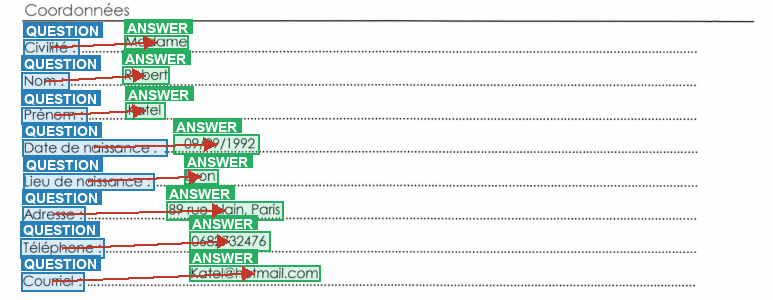
\includegraphics[width=\linewidth]{figures/linking_example_fr.png}
\end{minipage}
\caption{Top: FATURA field F1 of the zero-shot reader against BROS trained on $K$ templates (left); XFUND end-to-end link F1 (right; dots are seeds). Bottom: our finished BROS joint model, run locally on two unseen XFUND validation forms (German, French) through the OCR, word-splitting and windowing pipeline of the demo. Blue boxes are questions, green boxes answers, red arrows the predicted key-to-value links. German: six of seven links correct (birth date missed); French: eight links, each to the answer on its own line.}
\end{figure}

\section{Conclusions and what is missing}
A reader that must cite OCR lines handles new wording better than a tagger trained on 200 documents (76.5 vs 70.5), training wins once about 10 templates are seen and on dense tables, and for linking layout geometry helped (+5.9) where multilingual text did not ($-3.5$). Not run for lack of time: the fresh-set replication of prompt v2 (S32), the output-format test for the tuned VLM (S30), a learned router (S36 found up to $+5.8$ headroom on FATURA), and LayoutLMv3 on the hardest fold (Short-Form; still running at submission). Several analyses are post hoc; \texttt{STUDIES.md} flags each one.

\begingroup\footnotesize\setlength{\parindent}{0pt}
\begin{thebibliography}{9}\setlength{\itemsep}{0pt}\setlength{\parsep}{0pt}
\bibitem{bros} Teakgyu Hong, Donghyun Kim, Mingi Ji, et al. BROS: A Pre-trained Language Model Focusing on Text and Layout for Better Key Information Extraction from Documents, AAAI, 2022. \url{https://arxiv.org/abs/2108.04539}
\bibitem{lilt} Jiapeng Wang, Lianwen Jin and Kai Ding. LiLT: A Simple yet Effective Language-Independent Layout Transformer for Structured Document Understanding, ACL, 2022. \url{https://arxiv.org/abs/2202.13669}
\bibitem{vrdu} Zilong Wang, Yichao Zhou, Wei Wei, Chen-Yu Lee and Sandeep Tata. VRDU: A Benchmark for Visually-rich Document Understanding, KDD, 2023. \url{https://arxiv.org/abs/2211.15421}
\bibitem{docile} Štěpán Šimsa, Milan Šulc, Michal Uřičář, et al. DocILE Benchmark for Document Information Localization and Extraction, ICDAR, 2023. \url{https://arxiv.org/abs/2302.05658}
\bibitem{lmdx} Vincent Perot, Kai Kang, Florian Luisier, et al. LMDX: Language Model-based Document Information Extraction and Localization, arXiv, 2023. \url{https://arxiv.org/abs/2309.10952}
\bibitem{qwen} Qwen Team. \url{https://huggingface.co/Qwen/Qwen3-VL-8B-Instruct}, Accessed on: 22nd November, 2026.
\end{thebibliography}\endgroup
\end{document}
